\documentclass{standalone}
\usepackage{tikz}
\usepackage{caption}
\usepackage{subcaption}
\usepackage{helvet}
\usepackage{adjustbox}
\renewcommand{\familydefault}{\sfdefault}
\usetikzlibrary{
  positioning, calc, shapes.geometric, shapes.multipart, 
	shapes, arrows.meta, arrows, 
	decorations.markings, external, trees}

% Arrow style:
\tikzset{
    Arrow/.style = {
        thick, 
        decoration={
            markings,
            mark=at position 0.9999 with {
                \arrow[thick, #1]{latex}
                }
            }, 
        shorten >= 3pt, 
        preaction = {decorate}
    },
    Arrow/.tip={Triangle[length=2.5mm, width=2mm]},
    Arrow/.default={black}
}
% Text node
\tikzset{
Node/.style={
  text width=1cm,
  align=center,
  }
}
% Colors
\definecolor{aFill}{HTML}{2980b9}
\definecolor{yFill}{HTML}{ee5253}
\definecolor{uFill}{HTML}{bdc3c7}
\begin{document}
\begin{adjustbox}{width=20cm, height=12cm, keepaspectratio}
  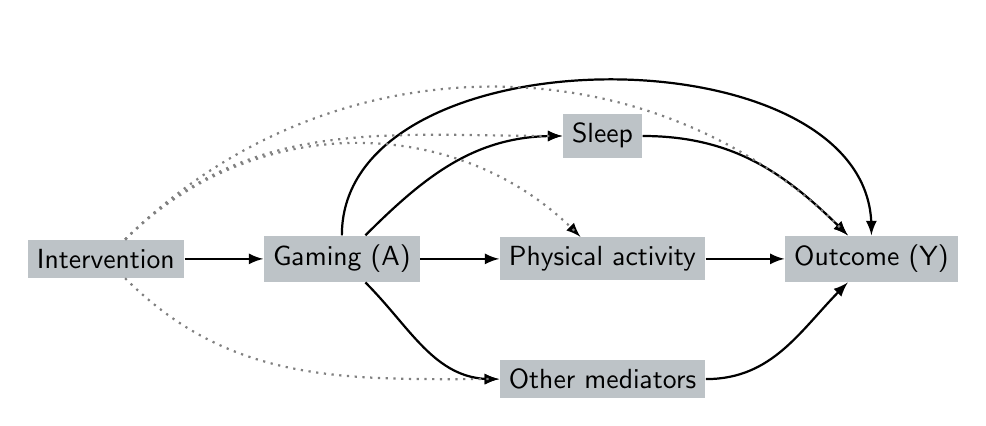
\begin{tikzpicture}
    \node[align=center, fill=uFill] (A) {Gaming (A)};
    \node[left=of A, fill=uFill] (I) {Intervention};
    \node[right=of A, fill=uFill,] (M0) {Physical activity};
    \node[above=of M0, fill=uFill] (M1) {Sleep};
    \node[below=of M0, fill=uFill] (M2) {Other mediators};
    \node[right=of M0, fill=uFill] (Y) {Outcome (Y)};
    \draw [Arrow] (I) to (A);
    \draw [Arrow] (A) to (M0);
    \draw [Arrow] (A) to [out=90, in=90] (Y);
    \draw [Arrow] (A) to [out=45, in=180] (M1);
    \draw [Arrow] (A) to [out=-45, in=180] (M2);
    \draw [Arrow] (M1) to [out=0, in=135] (Y);
    \draw [Arrow] (M2) to [out=0, in=-135] (Y);
    \draw [Arrow] (M0) to (Y);
    \draw [Arrow, dotted, color=gray] (I) to [out=45, in=135] (Y);
    \draw [Arrow, dotted, color=gray] (I) to [out=45, in=180] (M1);
    \draw [Arrow, dotted, color=gray] (I) to [out=45, in=135] (M0);
    \draw [Arrow, dotted, color=gray] (I) to [out=-45, in=180] (M2);

  \end{tikzpicture}
\end{adjustbox}
\end{document}